\documentclass{jsarticle}

\usepackage[margin=25.4truemm]{geometry}
\usepackage[dvipdfmx]{graphicx}

\title{1次元セルオートマトンで遊ぼう!}
\author{CottonTesseract}

\begin{document}
\maketitle
\section{はじめに}

\section{セルオートマトンとは?}
\emph{セルオートマトン}は、\emph{セル}と呼ばれる格子状の最小単位が多数並べられた計算モデルです。各セルは内部に\emph{状態}を持っており、\emph{近傍}のセルのと自身の現在の状態に基づいたシンプルな規則によって、次の自身の状態が決定されます。全てのセルは同じ規則を共有し、状態遷移は全てのセルで同時に起こります。

今回のプログラムでは、1980年代にスティーブン・ウルフラムによって研究された\emph{基本セルオートマトン}と呼ばれるものを扱っています。

\section{基本セルオートマトン}
基本セルオートマトンでは、セルは横1列に並べられ、セルは0と1という2つの状態を取ります。両側の隣接するセルが各セルの近傍となっており、状態は全てのセルで一斉に変化します。

では実際に試してみましょう。まず、\texttt{main.exe}を起動します。するとなにやらゴチャゴチャした小さなウィンドウと、空白のウィンドウが開きます。これらが開いたら、小さなウィンドウの下から2番目の「表示」というボタンをクリックします。すると空白のウィンドウに図\ref{fig:rule30_1px}のような模様が表示されます。

\begin{figure}[hbtp]
    \label{fig:rule30_1px}
    \centering
    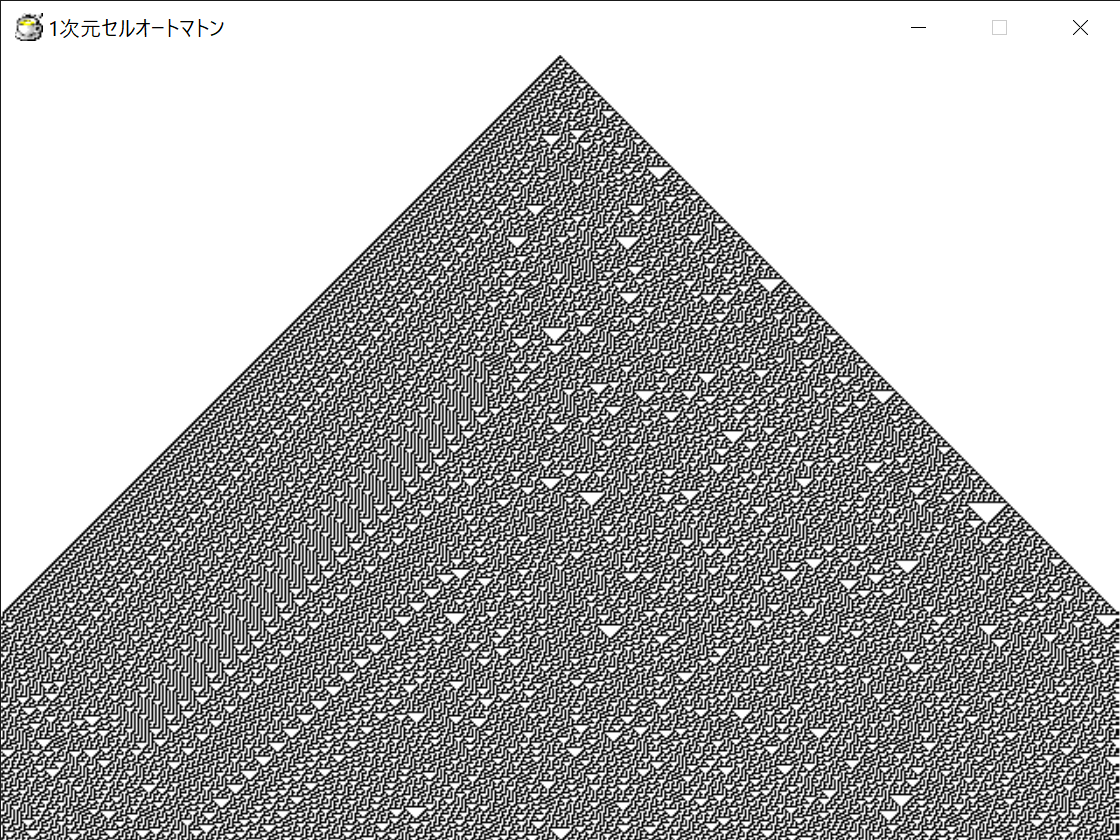
\includegraphics[width=8cm]{rule30.png}
    \caption{表示される模様}
\end{figure}

これは\emph{ルール30}と呼ばれる基本セルオートマトンの規則によって生成される模様です。白い四角形は状態0を取っているセル、黒は状態1のものを表しています。

横1列に並べられたセルの、遷移後の状態が次々と下に表示されていきます。これは鉄道の運行や素粒子の反応を表すダイアグラムと呼ばれる図とも似ています。

初期設定で表示するセルの大きさは1ですが、ここに別の数を指定することでセルの表示サイズを変更することができます。図\ref{fig:rule30_4px}はセルの表示サイズを4に設定した際のルール30です。

\begin{figure}[hbtp]
    \label{fig:rule30_4px}
    \centering
    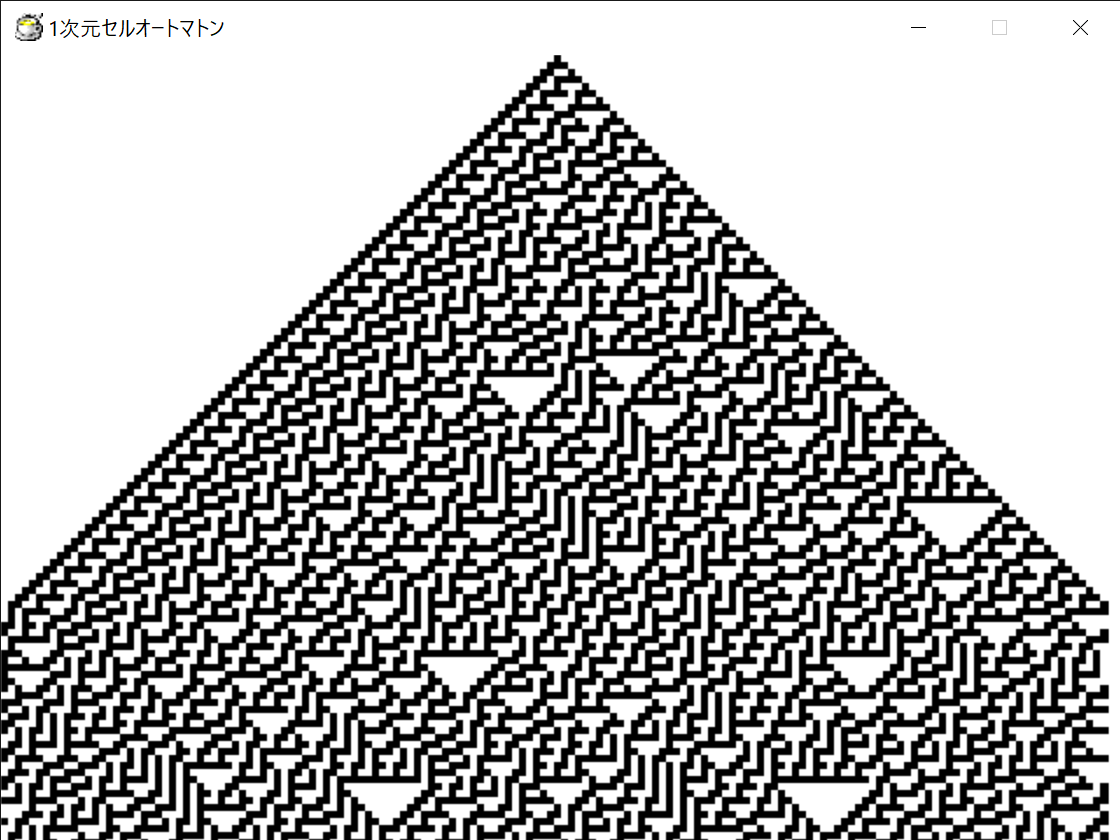
\includegraphics[width=8cm]{rule30_4.png}
    \caption{セルのサイズを4に設定した際のルール30}
\end{figure}

\end{document}
